\section{if-conversion的执行策略}

\subsection{if-conversion给编译器带来的挑战}

1997年,August在文章中详细讨论了处理器对谓词执行的支持给编译器带来的挑战,以及if-conversion的研究需要解决的问题\cite{August1997}。August指出,if-conversion的研究需要解决两个问题,一个是基本块的选择,如何选择基本块才能使得目标代码效率最高,另一个则是if-conversion执行时机的问题,在优化的早期执行if-conversion有利于向后面的过程暴露更多的潜在优化,而在编译的晚期进行if-conversion有利于的基本块的选取。

\subsection{August的基于逆向if-conversion的平衡算法}

August建议,在编译过程的早期大量应用if-conversion来发掘谓词执行带来的全部好处,此时形成的Hyperblock比目标体系能处理的大得多,然后在比较靠后的编译阶段进行部分逆向if-conversion,根据目标机器调整每个Hyperblock的谓词化代码的数量,以平衡控制流跟谓词数目。整个过程的工作流程如\fref{fig:ifcvtframework}所示。

\begin{figure}
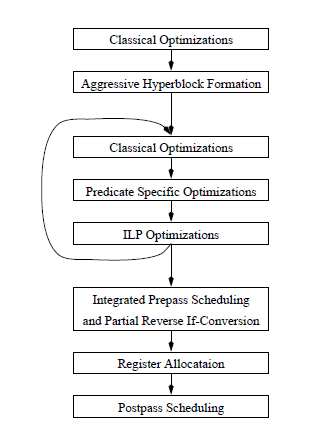
\includegraphics[width=\linewidth]{ifcvt-framework}
\caption{\label{fig:ifcvtframework} if-conversion的执行策略}
\end{figure}

\subsection{Hazelwood的动态if-conversion算法}

动态if-conversion的概念是Hazelwood在2000年提出的\cite{Hazelwood00alightweight},这里面的“动态”的意思是说,根据程序的运行情况来实时地对代码进行if-conversion。相比较动态if-conversion,之前的August的策略叫做静态if-conversion,因为所有的转换工作以及是否转换的决定已经在编译的时候就确定了。动态if-conversion的优点是,静态分析很难得出准确的分支预测失败概率,并且这些参数往往会随着程序的运行而改变,动态if-conversion可以随时调整程序到最佳状态以保证程序随时都能高效运行。Hazelwood的做法是,程序运行的过程中,动态监视程序的某些运行时参数,不如说分支命中率,分支预测失败惩罚等等,当这些参数达到某个阈值的时候,即对程序进行if-conversion,将相应的分支转换成谓词执行,当这些参数达到另一个阈值的时候,进行逆向if-conversion这样通过动态地对程序进行分支与谓词执行之间的转换,达到性能最优。